\documentclass{beamer}

\usepackage{amssymb}
\usepackage{amsfonts}
\usepackage{amsmath}
\usepackage{amsthm}
\usepackage{setspace}
\usepackage{longtable}
\usepackage{graphicx}
\usepackage{mathtools}
\usepackage{color}
\usepackage{array}
\usepackage{calc} 
\usepackage{bm}
\usepackage{caption}
\usepackage{float}

\usetheme{CambridgeUS}
\useoutertheme{infolines}
%numbering
\setbeamercolor{background canvas}{bg=white}
\setbeamersize{text margin left=1cm,text margin right=1cm}

\title[AI1110  Assignment-5]{ASSIGNMENT-5}
\subtitle{AI1110}
\author[]{MUKUNDA REDDY \\ AI21BTECH11021}
\date{}

\begin{document}
  \begin{frame}
      \titlepage
  \end{frame}
  
  \begin{frame}{Outline}
      \tableofcontents
  \end{frame}
  
  \section{Question}
  \begin{frame}{Example 4-3}
     In the coin-tossing experiment, the probability of
     heads equals $p$ and the probability
     of tails equals $q$. Find its distribution function $F(x)$ for every x' from  $-\infty$ to $\infty$ ? \\
  \end{frame}
  
  \section{Solution}
  \begin{frame}{Solution}
     Here $F(x)$  is called the cumulative distribution
     function of the random variable x.It is defined by
     \begin{equation}
     \label{definition}
     F_{\textit{x}} (w) = P\{ \textbf{X} \le \textit{w} \}    
     \end{equation}
     
     We define a random variable X such that
     \[
        X = 
     \begin{cases}
     1 & \text{if heads occured} \\
     0 & \text{if tails occured} \\
     \end{cases}
     \]
  \end{frame}
  
   \subsubsection{Case (i)}
      \begin{frame}{Case (i) : $x < 0$}
      To find cumulative distribution consider cases of x from $-\infty$ to  $\infty$. \\
      Given $x < 0$ but both $\{X(h) = 1\} ,\{X(t) = 0\} > x $  exceeds given interval of x so
      \begin{align}
      F(x) &= P\{X \le x \} \nonumber \\  
     &= P\{ \phi \} \: \text{(Null set)} \nonumber \\  
            &= 0 
      \end{align}
      \end{frame}
      
     \subsubsection{Case (ii)}
      \begin{frame}{Case (ii) : $0 \le x < 1$}
      Given $0 \le x < 1$. we know $\{X(h) = 1\} > x$ but  $\{X(t) = 0\} \le [0,1)$ Hence \\
      \begin{align}
      F(x) &= P\{X \le x \} \nonumber \\
        &=  P\{t\} \:, \forall x \in [0,1),X(t) \le x \nonumber \\
        &=  q 
      \end{align}
      
      \end{frame}
      
      
      \subsubsection{Case (iii)}
      \begin{frame}{Case (iii) : $ x \ge 1$}
      We have $\{X(h)=1\} \le x$ and $\{X(t)= 0\} \le x$ as
      here $x \in [1,\infty)$, also events $X(h)$ and $X(t)$
      are partition of sample space so $p+q = 1$.\\
      \begin{align}
          F(x) &= P(X \le x) \nonumber \\
            &= P\{t,h\} \:,\forall x \in [1,\infty),X(t,p) \le x \nonumber \\
            &= p+q  \nonumber \\
            &= 1 
      \end{align}
          
      \end{frame}
      
      \section{Cumulative Distribution Graph}
      \begin{frame}{Graph}
          \begin{figure}
              \centering
              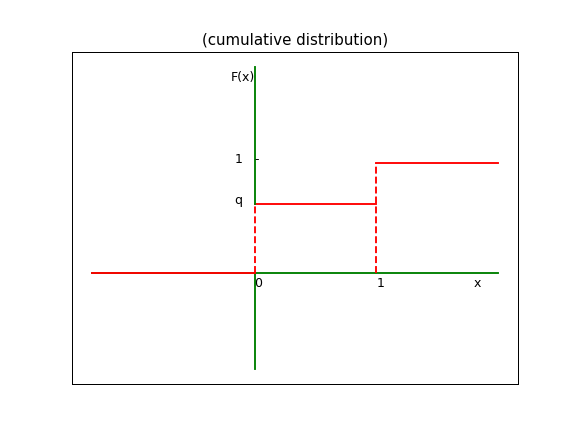
\includegraphics[scale=0.5]{Figure_1.png}
              \caption{Cumulative Distribution}
              \label{fig:my_CDG}
          \end{figure}
      \end{frame}
\end{document}
